%  LaTeX support: latex@mdpi.com 
%  In case you need support, please attach all files that are necessary for compiling as well as the log file, and specify the details of your LaTeX setup (which operating system and LaTeX version / tools you are using).

% You need to save the "mdpi.cls" and "mdpi.bst" files into the same folder as this template file.

%=================================================================
\documentclass[journal,article,submit,moreauthors,pdftex,10pt,a4paper]{Definitions/mdpi} 

% If you would like to post an early version of this manuscript as a preprint, you may use preprint as the journal and change 'submit' to 'accept'. The document class line would be, e.g. \documentclass[preprints,article,accept,moreauthors,pdftex,10pt,a4paper]{mdpi}. This is especially recommended for submission to arXiv, where line numbers should be removed before posting. For preprints.org, the editorial staff will make this change immediately prior to posting.

%
%--------------------
% Class Options:
%--------------------
% journal
%----------
% Choose between the following MDPI journals:
% acoustics, actuators, addictions, admsci, aerospace, agriculture, agronomy, algorithms, animals, antibiotics, antibodies, antioxidants, applsci, arts, asi, atmosphere, atoms, axioms, batteries, bdcc, behavsci, beverages, bioengineering, biology, biomedicines, biomimetics, biomolecules, biosensors, brainsci, buildings, carbon, cancers, catalysts, cells, ceramics, challenges, chemengineering, chemosensors, children, cleantechnol, climate, clockssleep, cmd, coatings, colloids, computation, computers, condensedmatter, cosmetics, cryptography, crystals, cybersecurity, data, dentistry, designs, diagnostics, dairy, diseases, diversity, drones, econometrics, economies, education, electrochem, electrochemistry, electronics, energies, entropy, environments, epigenomes, est, fermentation, fibers, fire, fishes, fluids, foods, forecasting, forests, fractalfract, futureinternet, galaxies, games, gastrointestdisord, gels, genealogy, genes, geohazards, geosciences, geriatrics, hazardousmatters, healthcare, heritage, highthroughput, horticulturae, humanities, hydrology, informatics, information, infrastructures, inorganics, insects, instruments, ijerph, ijfs, ijms, ijgi, ijtpp, inventions, j, jcdd, jcm, jcs, jdb, jfb, jfmk, jimaging, jof, jintelligence, jlpea, jmmp, jmse, jpm, jrfm, jsan, land, languages, laws, life, literature, logistics, lubricants, machines, magnetochemistry, make, marinedrugs, materials, mathematics, mca, medsci, medicina, medicines, membranes, metabolites, metals, microarrays, micromachines, microorganisms, minerals, modelling, molbank, molecules, mps, mti, nanomaterials, ncrna, neonatalscreening, neuroglia, nitrogen, nutrients, ohbm, particles, pathogens, pharmaceuticals, pharmaceutics, pharmacy, philosophies, photonics, plants, plasma, polymers, polysaccharides, proceedings, processes, proteomes, publications, quaternary, qubs, reactions, recycling, religions, remotesensing, reports, resources, risks, robotics, safety, sci, scipharm, sensors, separations, sexes, sinusitis, smartcities, socsci, societies, soilsystems, sports, standards, stats, surfaces, surgeries, sustainability, symmetry, systems, technologies, toxics, toxins, tropicalmed, universe, urbansci, vaccines, vehicles, vetsci, vibration, viruses, vision, water, wem, wevj
%---------
% article
%---------
% The default type of manuscript is article, but can be replaced by: 
% abstract, addendum, article, benchmark, book, bookreview, briefreport, casereport, changes, comment, commentary, communication, conceptpaper, correction, conferenceproceedings, conferencereport, expressionofconcern, meetingreport, creative, datadescriptor, discussion, editorial, essay, erratum, hypothesis, interestingimages, letter, meetingreport, newbookreceived, opinion, obituary, projectreport, reply, reprint, retraction, review, perspective, protocol, shortnote, supfile, technicalnote, viewpoint
% supfile = supplementary materials
% protocol: If you are preparing a "Protocol" paper, please refer to http://www.mdpi.com/journal/mps/instructions for details on its expected structure and content.
%----------
% submit
%----------
% The class option "submit" will be changed to "accept" by the Editorial Office when the paper is accepted. This will only make changes to the frontpage (e.g. the logo of the journal will get visible), the headings, and the copyright information. Also, line numbering will be removed. Journal info and pagination for accepted papers will also be assigned by the Editorial Office.
%------------------
% moreauthors
%------------------
% If there is only one author the class option oneauthor should be used. Otherwise use the class option moreauthors.
%---------
% pdftex
%---------
% The option pdftex is for use with pdfLaTeX. If eps figures are used, remove the option pdftex and use LaTeX and dvi2pdf.

%=================================================================
\firstpage{1} 
\makeatletter 
\setcounter{page}{\@firstpage} 
\makeatother
\pubvolume{xx}
\usepackage[]{algorithmic}
\issuenum{1}
\articlenumber{1}
\pubyear{2018}
\copyrightyear{2018}
\externaleditor{Academic Editor: name}
\history{Received: date; Accepted: date; Published: date}

%\updates{yes} % If there is an update available, un-comment this line
 
%------------------------------------------------------------------
% The following line should be uncommented if the LaTeX file is uploaded to arXiv.org
%\pdfoutput=1

%=================================================================
% Add packages and commands here. The following packages are loaded in our class file: fontenc, calc, indentfirst, fancyhdr, graphicx, lastpage, ifthen, lineno, float, amsmath, setspace, enumitem, mathpazo, booktabs, titlesec, etoolbox, amsthm, hyphenat, natbib, hyperref, footmisc, geometry, caption, url, mdframed, tabto, soul, multirow, microtype, tikz

%=================================================================
%% Please use the following mathematics environments: Theorem, Lemma, Corollary, Proposition, Characterization, Property, Problem, Example, ExamplesandDefinitions, Hypothesis, Remark, Definition
%% For proofs, please use the proof environment (the amsthm package is loaded by the MDPI class).

%=================================================================
% Full title of the paper (Capitalized)
\Title{Classification and Regression of Spatio-Temporal EMG Signals using NeuCube Spiking Neural Network and its implementation on SpiNNaker Neuromorphic Hardware}

% Author Orchid ID: enter ID or remove command
\newcommand{\orcidauthorA}{0000-0003-3257-0211} % Add \orcidA{} behind the author's name
\newcommand{\orcidauthorC}{0000-0002-6591-1118}
%\newcommand{\orcidauthorB}{0000-0000-000-000X} % Add \orcidB{} behind the author's name

% Authors, for the paper (add full first names)
\Author{Jan Behrenbeck $^{1}$, Zied Tayeb $^{2,3}$*\orcidA{}, Cyrine Bhiri $^{2}$,  Christoph Richter $^{2}$*\orcidC{}, Oliver Rhodes $^{4}$, Nikola Kasabov $^{5}$, Steve Furber $^{4}$, Gordon Cheng $^{3}$ and  J\"org Conradt $^{2}$}


% Authors, for metadata in PDF
\AuthorNames{Jan Behrenbeck, Zied Tayeb, Cyrine Bhiri, Christoph Richter,  Oliver Rhodes, Nikola Kasabov, Steve Furber, Gordon Cheng and J\"org Conradt}

% Contact information of the corresponding author
\corres{Correspondence: zied.tayeb@tum.de; Tel.: +49- 89 289 26791}

% Affiliations / Addresses (Add [1] after \address if there is only one affiliation.)
\address{%
$^{1}$ \quad Department of Mechanical Engineering, Technical University of Munich, Germany\\
$^{2}$ \quad Neuroscientific System Theory, Department of Electrical and Computer Engineering, Technical University of Munich, Germany\\
$^{3}$ \quad Institute for Cognitive Systems, Technical University of Munich, Germany\\
$^{4}$ \quad School of Computer Science, The University of Manchester, UK\\
$^{5}$ \quad Knowledge Engineering and Discovery Research Institute, Auckland University of Technology, AUT Tower, Level 7, cnr Rutland and Wakefield Street, Auckland 1010, New Zealand}

% Abstract (Do not insert blank lines, i.e. \\) 
\abstract{The third generation of neural networks, spiking neural network (SNN), aims to bridge the gap between neuroscience and machine learning using biologically plausible learning models. Due to their tremendous capability of capturing the spatio-temporal information encoded in time-series signals,  such networks have gained momentum over the last decades and are being widely used in pattern recognition and classification tasks. Notwithstanding the substantial advances that have been made in classifying surface electromyography signals (sEMG), the decoding algorithms still rely on hand-crafted features and vector-based learning. The extraction of such discriminative features slows down the computation, requires substantial computing resources and restricts the flexibility, the adaptability and the applicability of a system. In this context, this work investigates the use of the NeuCube spiking model to classify directly different grasp movements from raw EMG data as well as estimations of the applied finger forces. Experimental results reveal a better classification accuracy using the NeuCube model compared to traditional machine learning methods. We reached a validation accuracy of 85.5\%, a test accuracy of 81\% as well as less than 19\% of relative root mean square error (rRMSE) when estimating finger forces, using EMG data collected from four different human subjects. This work provides a proof of concept for a successful implementation of the NeuCube spiking model on the SpiNNaker neuromorphic platform for raw sEMG decoding.    
}

% Keywords
\keyword{Surface EMG (sEMG); NeuCube; Spiking neural networks; SpiNNaker neuromorphic platform; prosthetic hands.}

% The fields PACS, MSC, and JEL may be left empty or commented out if not applicable
%\PACS{J0101}
%\MSC{}
%\JEL{}

%%%%%%%%%%%%%%%%%%%%%%%%%%%%%%%%%%%%%%%%%%
% Only for the journal Applied Sciences:
\featuredapplication{A neuroprosthesis is a device that has a direct interface with the nervous system and supplements or substitutes functionality in the patient's body. Regarding the increasing consumer base of amputees, neuroprosthetic research has gained momentum over the last decades. However, current neuroprostheses still exhibit various drawbacks, such as high power consumption, low computational speed and consequently limited control capabilities. This work investigates the implementation of the NeuCube spiking algorithm to efficiently decode different hand poses and associated forces from sEMG signals without hand-crafted features. This spike-based neuronal processing algorithm yields significantly higher flexibility and inherent run-time adaptation, well beyond traditional hard-coded signal processing methods. In a parallel investigation, this work explores also the implementation of this decoding algorithm on dedicated neuromorphic hardware, which allows low-energy real-time processing to create portable closed-loop neuroprosthetic devices.}
%%%%%%%%%%%%%%%%%%%%%%%%%%%%%%%%%%%%%%%%%%

%%%%%%%%%%%%%%%%%%%%%%%%%%%%%%%%%%%%%%%%%%
\dataset{http://gumpy.org/}

%%%%%%%%%%%%%%%%%%%%%%%%%%%%%%%%%%%%%%%%%%
% Only for the journal Toxins
%\keycontribution{The breakthroughs or highlights of the manuscript. Authors can write one or two sentences to describe the most important part of the paper.}

%\setcounter{secnumdepth}{4}
%%%%%%%%%%%%%%%%%%%%%%%%%%%%%%%%%%%%%%%%%%
\begin{document}
%%%%%%%%%%%%%%%%%%%%%%%%%%%%%%%%%%%%%%%%%%
%% Only for the journal Gels: Please place the Experimental Section after the Conclusions

%%%%%%%%%%%%%%%%%%%%%%%%%%%%%%%%%%%%%%%%%%

\section{Introduction}
There has been a rapid rise in the use of EMG analysis for surface myoelectric signal pattern recognition, which is commonly investigated for the control of upper-limb prostheses, human-assisting robots, as well as  rehabilitation devices \cite{1}. Recent studies have focused on how to increase the level of comfort and effectiveness of these devices. Particularly, these studies have tended to focus on reducing the latency period between intention and the subsequent behavior. With regard to traditional approaches towards robust pattern recognition, the focus has always been on extracting hand-crafted features, which involves designing "engineering" features and feeding them into a classifier or a regressor \cite{2}. However, this technique becomes computationally demanding when classifying multiple hand gestures \cite{3} or decoding complex reach-to-grasp movements \cite{4}. Hence, it is not suitable for real-time prostheses control, where a very low latency is always required \cite{5}.
This work focuses on the decoding of four different hand poses, namely two-digit pinch, three-digit pinch, a fist and hand open from raw sEMG signals using the NeuCube spiking neural network \cite{6}. Additionally, a classic machine learning classifier has been implemented for benchmarking purposes. First, the spiking model was tested on a standard computer and was thereafter implemented on the SpiNNaker neuromorphic hardware \cite{7}. Such a hardware system offers a low power consumption, scalability and a competitive real-time capability, which could enhance online prostheses control.   
The implemented "brain-inspired" model comprises three stages: An encoding stage, which converts time-series signals into spike trains; a three-dimensional brain-shaped recurrent SNN reservoir, which learns spatio-temporal patterns from spatio-temporal EMG data; and an output classifier, which is trained on class-specific reservoir dynamics and predicts class labels for unknown samples. 
Overall, this  work  presents a  first  attempt  to  use the tremendous advantages of SNN models for sEMG decoding. In particular, the NeuCube was used to decode different hand gestures and associated forces from sEMG signals without hand-crafted features, and to the best of our knowledge, no similar work has been carried out before. Thus, this work argues that using deep learning of spatio-temporal EMG data with SNN can be further investigated to achieve a smooth, accurate and adaptive control of prosthetics for complex movements within a larger time window. 
The remainder of this paper is structured as follows: The first section provides an overview of previous work on EMG signal decoding using traditional machine learning methods as well as SNN approaches. The second section describes the sEMG signal processing and implementation details of the NeuCube model on a standard computer. The neuromorphic implementation of the NeuCube on SpiNNaker is described in Section 3. Obtained results for hand poses and force estimation from sEMG signals using the NeuCube model as well as traditional machine learning approaches are shown in Section 4. Finally, Section 5 enumerates the strengths and weaknesses of the used method and proposes possible future improvements.
 
%%%%%%%%%%%%%%%%%%%%%%%%%%%%%%%%%%%%%%%%%%
\section{Related work}
\subsection{EMG signal decoding algorithms}
This section provides a review of the different algorithms used to classify sEMG signals spanning from classic machine learning techniques to SNN approaches. In \cite{8}, the authors investigated the decoding of sEMG in the early stages of reach-to-grasp movements ("pre- reach-to-grasp") for prosthetic hand control. Five different grasp types were classified, namely precision disk, tripod, thumb-2 fingers, thumb 4 fingers, and ulnar pinch. In the paper, the authors showed that an accuracy of 90\% of the final grasp gesture was obtained $0.5\,\text{s}$ after the movement onset. In \cite{9}, the authors used the NeuCube spiking model to classify six different hand gestures, namely hand closed, hand open, wrist flexion, wrist extension, ulnar and radial deviation. Various feature-extraction techniques were investigated (Mean-absolute value (MAV), Wavelength (WL) and combined features). Overall, a classification accuracy of 95.3\% was reached and the authors showed that the spiking approach outperformed classic machine learning methods when using MAV features. It should be noted, however, that an accuracy of only 68.7\% was attained when classifying raw EMG data without hand-crafted features. Table 1 compares different studies for sEMG classification and summarizes the obtained results. For a more comprehensive survey, readers are referred to \cite{10}. 
\begin{table}[ht]
\caption{Comparison of different EMG classification studies and their achieved accuracy}
\label{table}
\definecolor{table}{RGB}{79, 129, 189}
	\centering
	\small
	\begin{tabular}{lcccc}
	
		\textbf{Reference  } 	&\textbf{Number of classes}  &\textbf{Extracted features} &\textbf{Classifier} &\textbf{Accuracy} \\ 
		\hline\hline \cite{11} &7 &RMS & Adaptive Fuzzy classifier (ANFIS) &86\% \\
		\hline \cite{12} &10 &RMS and WL &Linear discriminant analysis (LDA)&98.87\% \\
		\hline \cite{13}  &5& RMS & Support vector machine (SVM)& 73\% \\
		\hline \cite{14}  &6&MAV and WL &LDA&91.64\% \\
		\hline \cite{15} & 3& TD&Fuzzy logic (FL) &97\%\\
		\hline \cite{16} &4& MAV, WL and RMS& Artificial neural networks (ANN)&89.2\%\\	
		\hline \cite{17} &-& Time-Frequency (TF)& SVM&90\%\\
		\hline \cite{18} &4& TF& ANFIS &92\%\\
		\hline \cite{9} &6& MAV, WL& NeuCube &95.33\%\\
		\hline \cite{9} &6& Raw data& NeuCube &68.7\%\\
		\hline Our work &4& Raw data& NeuCube &85.79\%\\
		\hline& & & &
	\end{tabular} 
\end{table}
%
\subsection{NeuCube applications}
The NeuCube model has been successfully applied and evaluated in several studies. In the context of electroencephalography (EEG) signal classification, the system was tested to model peri-perceptual brain processes from EEG signal \cite{19}. Doborjeh \textit{et al.} tested the model in a similar study on fMRI data \cite{20}. Chen \textit{et al.} and Taylor \textit{et al.} performed two feasibility studies for the use of NeuCube for motor-imagery based brain-computer interfaces (BCI) resulting in accuracy values of up to 81\% for recognition of wrist flexion, extension, and rest \cite{21,22}. NeuCube provides generally higher performance than traditional classifiers, which shows the potential of the model \cite{9}. 
Due to the good results in EEG-BCI studies, the NeuCube algorithm has been also adapted and has been successfully applied to other applications, such as traffic and sleep data \cite{23}, earth quake data \cite{24} as well as to perform ecological forecasts \cite{25}.
These positive results motivated our choice of using the NeuCube spiking algorithm for this study. 
%
\subsection{SpiNNaker neuromorphic hardware applications}
SpiNNaker is  a  massively- parallel  hardware system, inspired by the human  brain, which allows the emulation of large number of neurons  in  a biologically  plausible fashion \cite{7}.
The SpiNNaker board has already been applied in robotic contexts and connected to other neuromorphic hardware such as the eDVS silicon retina sensor to control an autonomous mobile robot, which can identify and approach a signal in real-time \cite{26}. In other works,  SpiNNaker was used to control a musculoskeletal robot in real-time \cite{27} as well as decoding motor imagery movements from EEG signal \cite{28}. Furthermore, SpiNNaker was used for audio samples \cite{29} and handwritten digits classification \cite{30}.
%%%%%%%%%%%%%%%%%%%%%%%%%%%%%%%%%%%%%%%%%%%%%%%%%%%%%%%%%
%%%%%%%%%%%%%%%%%%%%%%%%%%%%%%%%%%%%%%%
\section{Materials and Methods}
\subsection{EMG signals recording}
EMG data were recorded from four different subjects: three right-handed males and one left-handed female. Subjects were between 22 and 24 years old and claimed to have no record of neurological disorders. Before this study, they had never performed tasks involving myoelectric control of any external devices. Subjects were recruited to perform a series of hand movements, namely 2-digit grasp, 3-digit grasp, fist and hand open. The grasping tasks were performed on an easy to grasp cylindrical object as shown in Figure \ref{FIG:EXPERIMENTAL_PARADIGM}. Each trial consisted of five seconds of movement execution followed by a five-second break. During each trial, the subject was asked to perform one of the four postures, which were selected from a discrete uniform distribution, with two levels of force (high, low). Data used in this example study as well as the experimental paradigm are made publicly available with the gumpy toolbox \cite{31}. To measure the applied force, force sensing resistors (FS402) were placed on the fingertips, a voltage divider and an Arduino Uno \cite{32} were used to acquire the global force value, which was set as the sum of each individual measured finger force. EMG data were recorded and sampled at 512\,Hz using a g.USBamp system \cite{33}. Four pairs of electrodes, which cover the muscles of the forearm in a ring-like fashion were used, and the reference electrode was placed on the elbow bone. 
\begin{figure}[H]
    \centering
    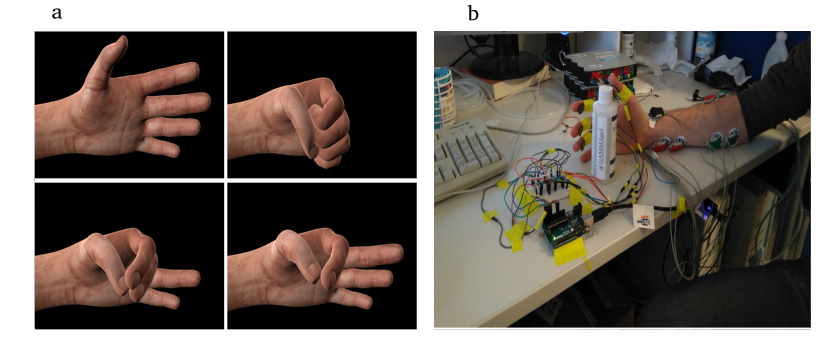
\includegraphics [width=0.8\linewidth]{EXPERIMENTAL_PARADIGM.png}
    \caption{ EMG recording paradigm. (a) Different hand gesture renderings prompting subjects.  (b) Recording setup of EMG signals during grasp movements.
}
    \label{FIG:EXPERIMENTAL_PARADIGM}
\end{figure}

\subsection{Data preprocessing}
EMG signals were processed using the gumpy.signal module in the gumpy BCI toolbox \cite{31}. EMG signals were band-pass filtered between 20 and 255\,Hz  using a 4th order zero-phase Butterworth filter and notch filtered at 50\,Hz  to remove the power line interference. Afterwards, EMG signals were normalized by the maximum voluntary isometric contraction (MVIC) magnitude. In addition, the computed mean of the signal was subtracted from each channel and then divided by the standard deviation. An example of a recording-session showing EMG signals and force intensity is depicted in Figure \ref{FIG:TwoFiguresFile.png}.  
\begin{figure}[H]
    \centering
    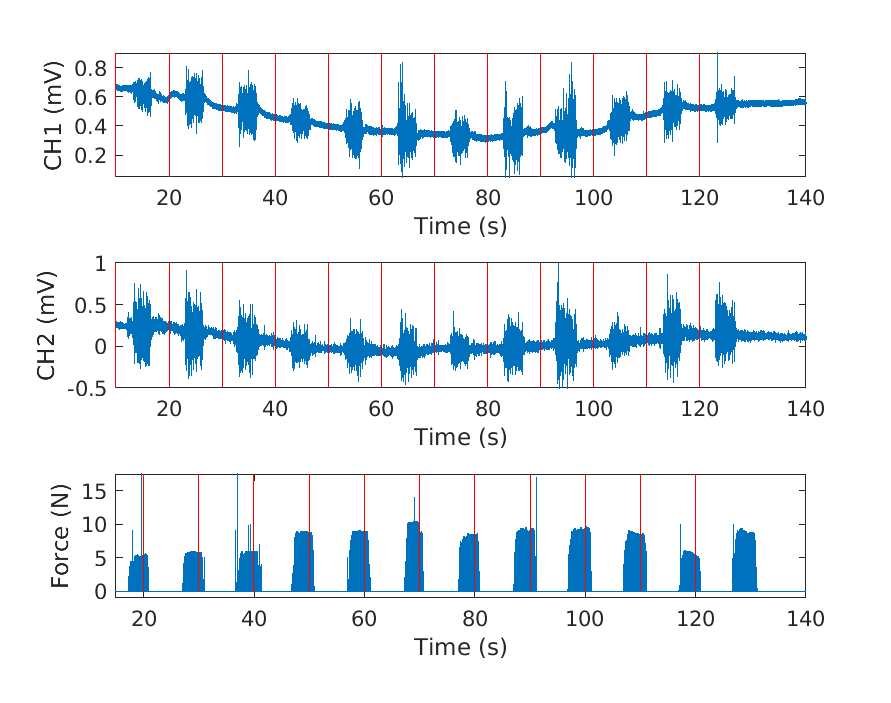
\includegraphics [width=0.8\linewidth]{TwoFiguresFile.png}
    \caption{Example of preprocessed EMG signals recorded  from two bipolar channels and the measured force intensity for 12 trials. CH1 and CH2 represent the first and the second EMG bipolar channels, respectively.
}
    \label{FIG:TwoFiguresFile.png}
\end{figure}

\subsection{NeuCube}
The mechanism of neuronal communication can be rebuilt through mathematical models to help create more efficient solutions to pattern recognition when it comes to complex and large signals such as spatial-/spectral-temporal data (SSTD). NeuCube is a 3-D SNN reservoir biologically inspired by the human brain that can be used to perform both classification and regression tasks on complex signals, which was proposed by N. Kasabov \cite{6}. At its core, NeuCube has some similarities with a liquid state machine \cite{34}, but it differs from it in many aspects: the structure is brain-inspired; mapping of input variables typically preserves their spatial location; and both unsupervised and supervised learning is applied. The NeuCube architecture comprises two basic parts, a recurrent SNN reservoir, also called SNNcube, and a readout function which is also realised as an SNN. It performs pattern recognition as follows: First, a spatio-temporal (or temporal) input signal \textit {x(t)} within a time window is acquired and encoded with some encoding function  $\mathrm{\textit {e}} : \mathbb{N} \times \mathbb{R}^\mathrm{\textit{n}} \rightarrow \mathbb{N} \times \mathbb{B}^\mathrm{\textit{n}}$ into a discrete time series of binary spikes, known as spike trains. Afterwards, the SNNcube is stimulated with the input spike train and learns the interaction between the input signals in an unsupervised mode. The SNNcube creates spatio-temporal patterns of connections as a result of this learning. The learned spatio-temporal patterns are transferred into another signal using a function $\mathrm{\textit{l}} : \mathbb{N} \times \mathbb{B}^\mathrm{\textit{n}} \rightarrow \mathbb{N} \times \mathbb{B}^\mathrm{\textit{p}}$, which integrates the spiking dynamics of the SNNcube. Due to the internal structure and properties of the SNNcube, different input samples induce different dynamic reactions in the SNNcube that are captured by a function $\mathrm{\textit{s}} : \mathbb{N} \times \mathbb{B}^\mathrm{\textit{p}} \rightarrow \mathbb{R}^\mathrm{\textit{p}}$ creating a spatio-temporal pattern of connectivity for each input sample. Finally, a readout function $\mathrm{\textit{r}} : \mathbb{R}^\mathrm{\textit{p}} \rightarrow \{0,1,...\mathrm{\textit{N}}\}$ is trained on the spatio-temporal patterns activated in the SNNcube by the input data samples to represent N input classes. In the end, NeuCube can predict the class $c$ of a new input signal $\textit{x}$ as $\textit{c(x)} = \mathrm{\textit{r(s(l(e(}x))))}$. Figure \ref{FIG:diagram4.pdf} provides an overview of NeuCube's modules and how they were used for EMG hand pose classification. More information about the NeuCube architecture can be obtained from \cite{6, 35, 36}.
\begin{figure}[H]
    \centering
    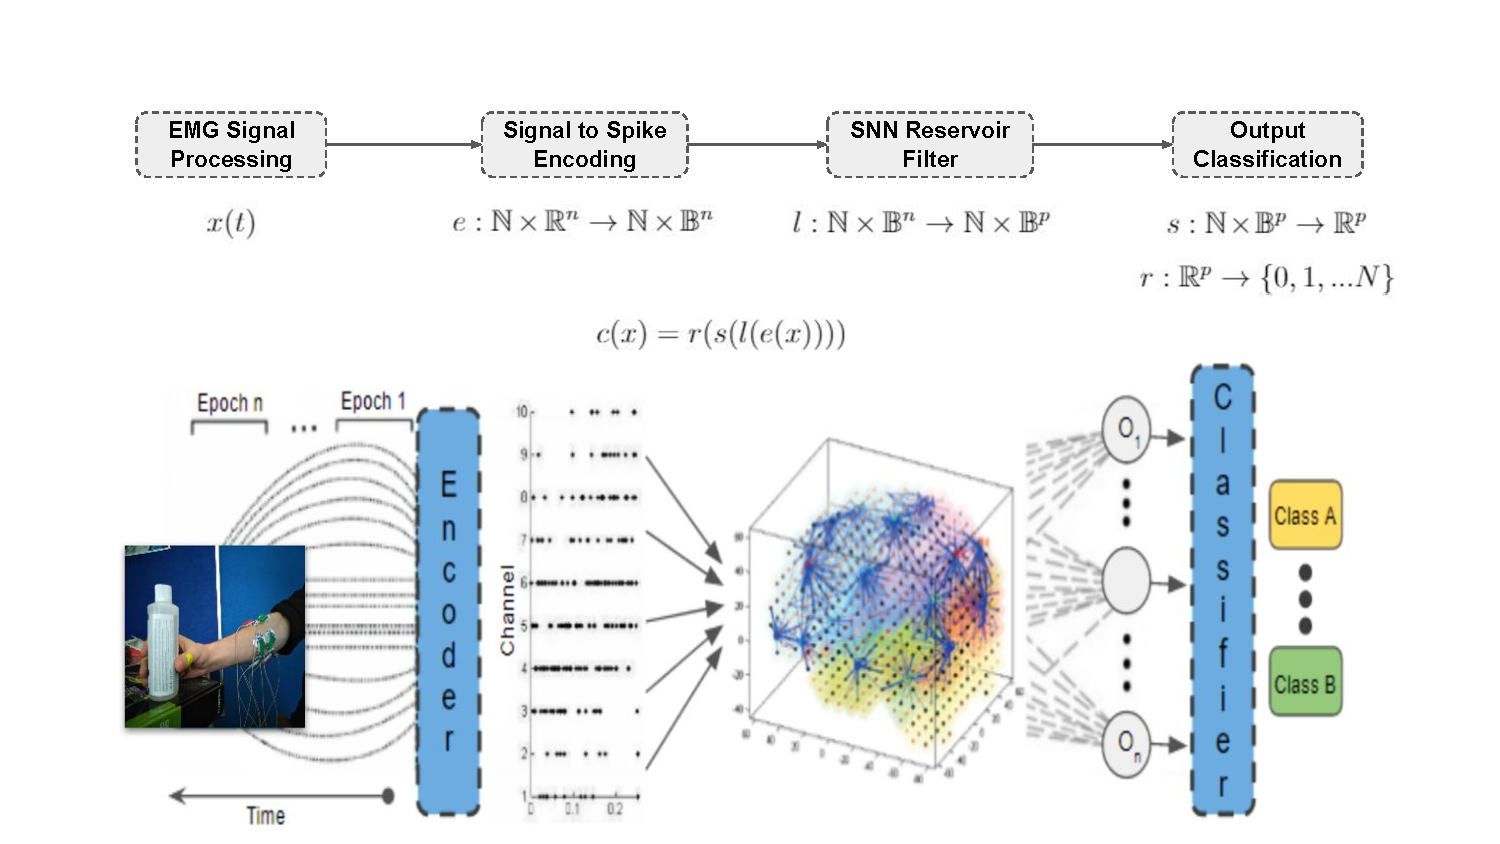
\includegraphics [width=0.9\linewidth]{diagram4.pdf}
    \caption{NeuCube's structure and its different modules used for EMG signal classification [adapted from \cite{6}]
}
    \label{FIG:diagram4.pdf}
\end{figure}

\subsubsection{EMG signal encoding}
To encode EMG time-continuous values into spike trains, a temporal difference (TD) algorithm was used. The algorithm works as follows:
Every time step $\tau$, the difference $\Delta v = v(\tau) - v(\tau-1)$ between the current and the previous value in the EMG signal is calculated and compared to a threshold. If the absolute difference exceeds the threshold, a spike is generated. The sign of the difference $\Delta v$ defines the sign of the spike and thereby its mode: If the spike is excitatory, the signal rises (+1), if the spike is inhibitory, the signal falls (-1) and if the absolute difference is smaller than the threshold, there is no spike (0). The pseudo-code for the TD- encoding algorithm is shown below. 

\ \\
Pseudo-code for TD-Encoding:
\begin{algorithmic}[1]
%\SetAlgoLined
\STATE \textit{spike\_train} = [ ]
\vspace{0.2cm}
\STATE \textit{last\_value} = 0
\vspace{0.2cm}
\FOR{time step $\tau$ in signal duration}
\vspace{0.1cm}
\STATE \textit{diff} = \textit{current\_value} - \textit{last\_value}
\vspace{0.2cm}
\IF{abs (\textit{diff}) $\ge$ threshold}
\vspace{0.2cm}
\STATE \textit{spike\_train}.add (sign (\textit{diff}) $\times$ time step $\tau$)
\vspace{0.2cm}
\ENDIF
\vspace{0.2cm}
\STATE \textit{last\_value} = \textit{current\_value}
\vspace{0.2cm}
\ENDFOR
\end{algorithmic}
\\
In this work, the optimum threshold for EMG signal was found to be 0.25  $\times$ variance (input\_signal). Furthermore, to evaluate the performance of the encoder and ensure the preservation of information in the signal, the encoded spike trains are decoded again and the reconstructed signals are compared to the original signals. The TD decoder works as follows: For every spike in the spike train, all the values in the signal after the spike time change by the threshold value depending on the mode of the spike. If the spike is excitatory, the signal rises. If the spike is inhibitory, the signal falls. The pseudo-code for the decoding algorithm  is described below. 

\ \\
Pseudo-code for TD-Decoding:
\begin{algorithmic}[1]
\STATE \textit{signal} = zeros (signal\_duration)
\vspace{0.2cm}
\FOR{\textit{spike} in spike\_train}
\vspace{0.1cm}
\IF{\textit{spike} is excitatory}
\vspace{0.2cm}
\STATE \textit{signal} [spike time $\tau$ : end] += threshold
\vspace{0.2cm}
\ELSE
\vspace{0.2cm}
\STATE \textit{signal} [spike time $\tau$ : end] -= threshold
\vspace{0.2cm}
\ENDIF
\vspace{0.2cm}
\ENDFOR
\end{algorithmic}
\\
%%%%%%%%%%%%%%%%%%%%%%%%%%%%%%%%%%%%%%%%%%%%%%%%%%%%%%%%
\vspace{0.2cm}
Other algorithms for data encoding into spikes and decoding can be found in \cite{35}. A widely used algorithm is the Ben's Spiker Algorithm (BSA) developed by Schrauwen \textit{et al.} \cite{37}.
The BSA uses solely excitatory spikes and makes use of a finite impulse response (FIR) reconstruction filter. It works as follows: Every instant in time $\tau$ two error metrics are calculated: 
\begin{equation}
    \mathrm{\textit{error}}_1 = \sum\nolimits_{i=0}^\mathrm{M} \mathrm{abs}(\mathrm{Signal}\textsubscript{ori}(i+\tau)-\mathrm{h}(i))
    \label{EQ:BSA_error_1}
    \end{equation}
\begin{equation}
    \mathrm{\textit{error}}_2 = \sum\nolimits_{i=0}^\mathrm{M} \mathrm{abs}(\mathrm{Signal}\textsubscript{ori}(i+\tau))
    \label{EQ:BSA_error_2}
    \end{equation}
with Signal\textsubscript{ori} being the original signal, h is the FIR filter window function, and M is the filter size.\\
If the first error metric is smaller than the second minus a threshold, a spike is generated and the filter is subtracted from the input signal; otherwise no spike is emitted. 
\subsection{NeuCube initialization and training}
In our implementation, the spiking neurons in the 3D SNNcube are spatially located according to a brain template, such as the Talairach stereotactic atlas \cite{38} by setting 1471 leaky integrate-and-fire (LIF) neurons each representing $1\,\text{cm}^3$ of brain tissue. In terms of number of neurons the initialization of the SNNcube is scalable from hundreds to hundreds of millions of neurons \cite{6} . A visualization of the input neurons matching the number (4) of bipolar channels is presented in Figure \ref{FIG:NeuCube_ini.png}. After the neurons are positioned, the synaptic connections are initialized in a small world connectome (SWC), which means that close neurons are connected with a higher probability than neurons that are further apart \cite{6}. For every neuron pair N$_i=(x_i,y_i,z_i)$ and N$_j=(x_j,y_j,z_j)$, the Euclidean distance is computed as $d_{i,j} = \sqrt{(x_i-x_j)^2+(y_i-y_j)^2+(z_i-z_j)^2}$.  Then, for each neuron pair, a connection probability $P_{i,j}$ is calculated according to Equation~\ref{EQ:conn_prob}. 
\begin{equation}
    P_{i,j} = \begin{cases}
    \mathrm{C} * \mathrm{e}^{-(d_{i,j}/\lambda)^2} & \mathrm{if}\; d_{i,j} \leq  \mathrm{d\textsubscript{thresh}}\\
    0 & \mathrm{otherwise}
    \end{cases}
    \label{EQ:conn_prob}
    \end{equation}
with C specifying the maximum connection probability, d\textsubscript{thresh} representing the maximum relative distance for connected neurons and $\lambda$ defining the small world connection radius. A $\labmda$ of 2.5\,mm was found to be the most effective for the 3D cube initialization. The model was trained in an unsupervised fashion using the Spike Timing Dependent Plasticity (STDP) mechanism \cite{39} with the hyperparameters shown in Figure \ref{FIG:NeuCube_ini.png}. 
\begin{figure}[H]
    \centering
    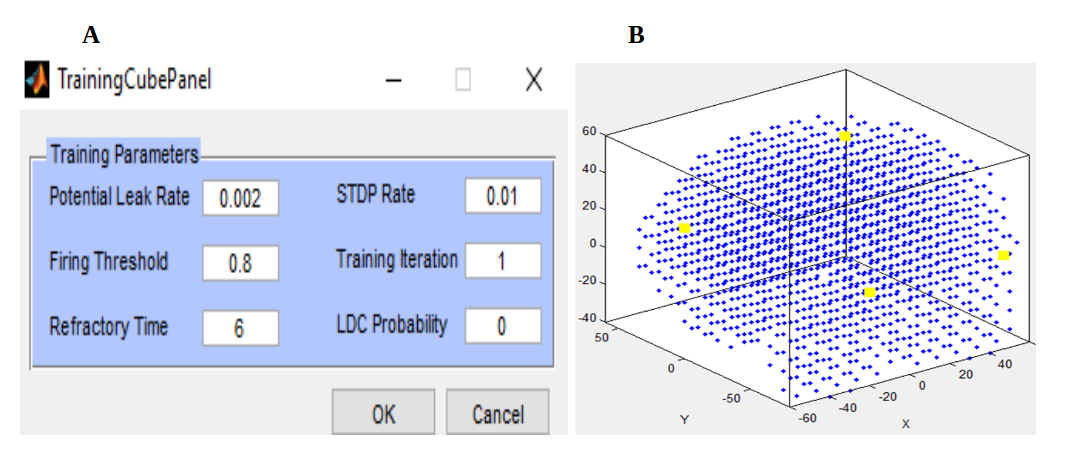
\includegraphics [width=0.8\linewidth]{NeuCube_ini.png}
    \caption{NeuCube initialization. A) Snapshot of the chosen hyperparameters for the NeuCube training model. B) EMG acquisition site locations in the NeuCube model representing the number of used EMG channels, where neuron positions are shown in blue and the EMG acquisition sites are shown in yellow. 
}
    \label{FIG:NeuCube_ini.png}
\end{figure}
Figure \ref{FIG:cube_tr.png} shows the SNNCube after training, which highlights the connections in terms of temporal relationships between the four electrodes. The blue color represents a positive neurons connection whereas the red represents a negative one. Additionally, the line thickness in Figure \ref{FIG:cube_tr.png} represents weight values, which highlights strong connections in the EMG acquisition sites. Last, it is important to mention that brighter neurons in the Figure \ref{FIG:cube_tr.png}  has stronger connections with other neurons than a dark neuron.
\begin{figure}[H]
    \centering
    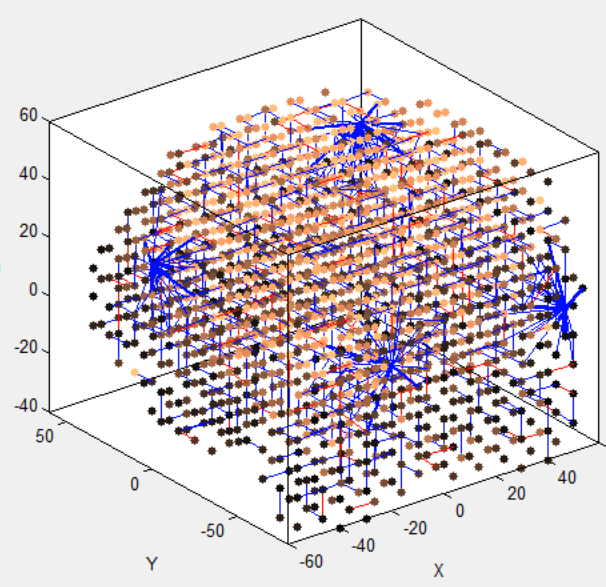
\includegraphics [width=0.55\linewidth]{cube-tr.png}
    \caption{A snapshot of the connections in the SNN cube after the unsupervised learning. The connections represent spatial-
temporal relationships between input data variables over time.
}
    \label{FIG:cube_tr.png}
\end{figure}
Overall, NeuCube applies the STDP learning to strengthen synapses that are involved in the creation of class-specific neuronal connectivity sets and weakens connections that take no role in class-specific neuron pattern creation. Thereby, discriminative spatio-temporal correlations are amplified and isolated. Interestingly, the spatially meaningful neuron structure and its complex connectivity enable the SNNcube to filter class-specific spatio-temporal features from EMG data by creating class-specific sets of firing neurons and isolating these sets with STDP-learning as shown in the example in Figure \ref{FIG:neuCUBE.png}. The learned input patterns can be as deep as needed in terms of time points that are measured for every sample. In our experiments we have used 200 time points for each sample, represented by $\sim 400$ milliseconds of EMG data. How deep in time the learned patterns should be depends on the task and the size of the SNNcube. There is no limit in principle, meaning that an SNNcube can learn longer time sequences, e.g. minutes, representing complex movements. This is a dramatic departure from the traditional EMG machine learning methods that use feature-vector based learning.        
\begin{figure}[H]
    \centering
    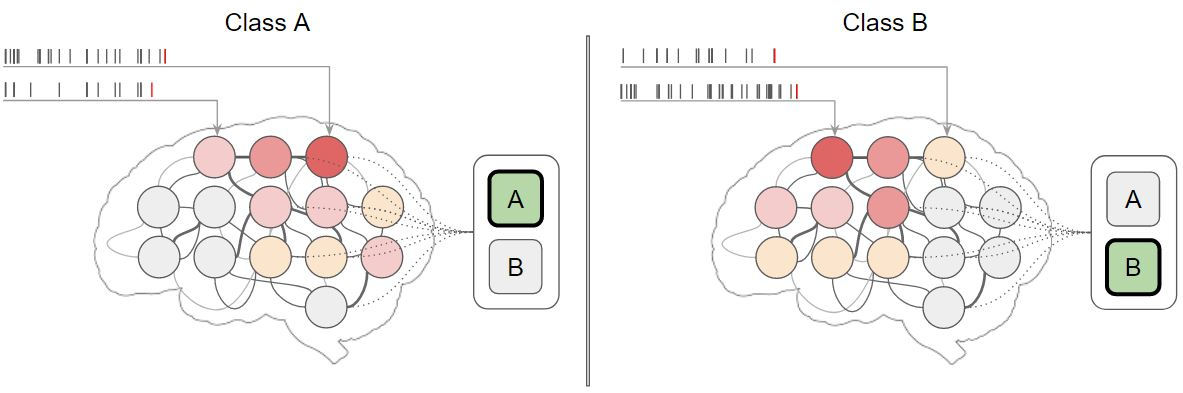
\includegraphics [width=0.9\linewidth]{neuCUBE.png}
    \caption{Schematic reservoir behavior. Due to the defined structure the 3D SNNcube that acts as a high dimensional space different input signals cause activity in different sets of neurons that results in created sets of connectivity. These sets represent the respective classes and can be used for classification.
}
    \label{FIG:neuCUBE.png}
\end{figure}

\subsection{Classification Module}
The third stage realizes a classification/regression function $\mathrm{\textit{s}} : \mathbb{N} \times \mathbb{B}^\mathrm{\textit{p}} \rightarrow \mathbb{R}^\mathrm{\textit{p}}$, which converts the activity of the SNNcube into output classes using readout function $\mathrm{\textit{r}} : \mathbb{R}^\mathrm{\textit{p}} \rightarrow \{\textit{0,1},...\mathrm{\textit{N}}\}$, which is trained with and finally classifies the state vectors. In this stage, dynamic evolving SNN (deSNN) \cite{40} was used due to its efficiency in spatial and temporal pattern recognition as well as its accurate spatial-temporal event prediction. Overall, the deSNN network is based on the comparison between the synaptic weights of a newly created output neuron that represents the new spatial-temporal pattern for recall, and the connection weights of the existing neurons created during training. The new input pattern is associated with the closest output neuron based on the minimum distance between the weight vectors. As the synaptic weights are dynamic, the distance will be calculated with both the initial weight vectors $\textit{w(0)}$ and connection weight vectors $\textit{w(T)}$ learned during training and recall. 
In order to validate the accuracy of the classifier/regressor, here, a three-fold cross validation was performed and the deSNN was trained in a supervised learning mode to classify different dynamic patterns of the reservoir output activities, which represent different spatio-temporal input data patterns from the different EMG classes. Obtained results are summarized in Section 5. 
%%%%%%%%%%%%%%%%%%%%%%%%%%%%%%%%%%%%%%%%%%%%%%%%%%%%%%%%%%%%
\section{Implementation of NeuCube on SpiNNaker}
This section describes the implementation of the NeuCube model on SpiNNaker and its motivation.

\subsection{Motivation and Neuromorphic hardware architecture}
NeuCube is a specialized, biologically inspired liquid state machine for modelling and recognition of complex spatio-temporal signal correlations using a network of spiking neurons. The execution of such artificial networks in real-time means simulating the asynchronous spiking behavior and synaptic communication between thousands of neurons simultaneously. However, simulating SNNs on standard computers requires substantial  computational overhead \cite{41}, largely annihilating the benefits of using spiking models in certain applications, such as prosthetics control. Neuromorphic computers are hardware systems \cite{41} developed specifically to simulate large networks of spiking neurons in real-time with low energy consumption often by collocating memory and processing. Thus, they achieve a speedup and support massively parallel data exchange in a brain-inspired fashion. 
We utilized the cross-platform high-level language PyNN\cite{42} to implement the NeuCube algorithm on the SpiNNaker platform. SpiNNaker \cite{7} uses a highly-parallel architecture to simulate large SNNs efficiently. This hardware system relies on regular microprocessors to maintain the flexibility and scalability of ordinary computers and at the  same time avoid the Von Neumann Bottleneck when simulating large numbers of neurons. A 4-node
SpiNNaker board depicted in Figure \ref{FIG:spiNNaker-baord.png} consisting of 64 processors and capable of simulating up to 10,000 neurons, was sufficient to suit the size of our network. In fact, our choice of using the small SpiNNaker board was highly motivated by its compact size, its power efficiency, thereby its suitability to be integrated later on, in a prosthetic device. 
%Last, we wish to mention that despite such advantages of neuromorphic computing, the use of spiking models on neuromorphic systems to decode time-series signals has been rarely investigated \cite{28, 41}.

%This either requires hardware that is capable of massive parallel processing or software that can simulate parallel processes. Neuromorphic hardware \cite{25} has been developed specifically to simulate large networks of spiking neurons in real-time with low energy consumption. Thus, neuromorphic systems have become more popular for for  being highly  connected, offering massively parallel architecture with low power consumption, and collocating  memory  and  processing. 

%In addition, to embed the hardware in mobile applications and enable an independent, off-grid power supply requires low power consumption. Standard hardware, such as Central Processing Units (CPUs), Graphical Processing Units (GPUs), or Field Programmable Gate Arrays (FPGAs), do not satisfy these conditions, because they either consume too much energy or are not able to run complex simulations of SNN in real-time. Neuromorphic hardware \cite{25} has been developed specifically to simulate large networks of spiking neurons in real-time with low energy consumption. 

\begin{figure}[H]
    \centering
    \includegraphics [width=0.55\linewidth]{spiNNaker-baord.png}
    \caption{The 4-node SpiNNaker chip
}
    \label{FIG:spiNNaker-baord.png}
\end{figure}
%%%%%%%%%%%%%%%%%%%%%%%%%%%%%%%%%%%%%%%%%%%%%%%%%%%%%%%%
\subsection{Implementation details}

The NeuCube was implemented using the open source Python package for neural networks specification PyNN \cite{42}. In addition, the KNeighborsClassifier class from the SciKit-Learn library \cite{43} was used as part of the deSNN implementation. The implementation comprises three stages: an encoding stage, which converts sEMG signals into spike trains; a three dimensional brain-shaped recurrent Spiking Neural Network reservoir, which learns spatio-temporal correlations from the data; and an output classifier, which is trained on class-specific reservoir dynamics and predicts class labels for unknown samples. 
%%%%%%%%%%%%%%%%%%%%%%%%%%%%%%%%%%%%%%%%%%%%%%%%%%%%%%%%%
%\subsubsection{Implementation of stage 1: Signal to Spike Encoding}
The spike encoding stage has been implemented in Python and runs on the host computer. It converts normalized EMG samples into sets of spike trains. It should be noted that the TD algorithm described in Section 3.3.1 was chosen and implemented. 
%\subsubsection{Implementation of stage 2: SNN Reservoir}
The 3D reservoir implementation was split into two parts: the generation of the network structure; and the simulation of the network, which includes both training and classification. The network generation, meaning the positioning and connection of neurons, was executed on the host computer. Thereafter, the network was mapped and trained on a SpiNNaker machine using the sPyNNaker software \cite{44}. 
%We wish to mention that the Talairach stereotactic brain atlas described before in Section 3.4, was used for positioning the neurons. 
%\subsubsection{Implementation of stage 3: Output classification}
The third stage employs a modified version of the deSNN algorithm described in Section 3.5 for the final classification task and can be separated into network generation and sample classification. Stage 3 runs on the host computer. First, each neuron in the output stage is connected to each reservoir neuron of the second stage. The weights are initially calculated using the rank order (RO) rule \cite{45} and are adjusted using the spike driven synaptic plasticity (SDSP) rule \cite{46}. As a result, every output neuron contains three feature vectors of 1471 elements (the total number of reservoir neurons) based on its connections to the reservoir neurons: one for the initial weights, one that contains the total number of spikes on each synapse, and one for the final weights. These weight vectors represent the feature vectors, which are used as inputs to train a KNN classifier from the SciKit-Learn library \cite{43}. 

%%%%
\section{Results}
\subsection{Hand pose recognition}
\subsubsection{Off-line results}
In this section, we show the obtained NeuCube classification results of four hand movements recorded from four different subjects. To benchmark our obtained results, we compared the obtained results with the K-nearest neighbor algorithm (KNN) using two different feature-extraction methods namely mean absolute value (MAV), root-mean square (RMS) as well as with raw data directly. Through all subjects, a mean accuracy of  $(85.2\pm 1.5)\%$ was achieved using NeuCube on raw EMG data. Interestingly, the NeuCube model outperforms the KNN algorithm by a large margin (30\%) while classifying the raw data. Overall, the obtained results confirm the evidence proposed before in \cite{9}, which shows that pattern recognition with standard machine learning algorithms does not perform as well in classification tasks without hand-crafted features. Thus, it reinforces the usefulness of using SNN algorithms, and in particular the NeuCube model when working directly with raw data. More importantly, the obtained results for classifying raw EMG data are better compared to the similar work presented before in \cite{9}, where an overall accuracy of only 68\% was reached for classification of six hand movements collected from a single subject. Results are depicted in Figure \ref{FIG:x.pdf}. It should be noted that balanced accuracy was chosen as an evaluation metric for the trained model and a stratified 3-fold cross-validation was performed during the validation phase. 
\begin{figure}[H]
    \centering
    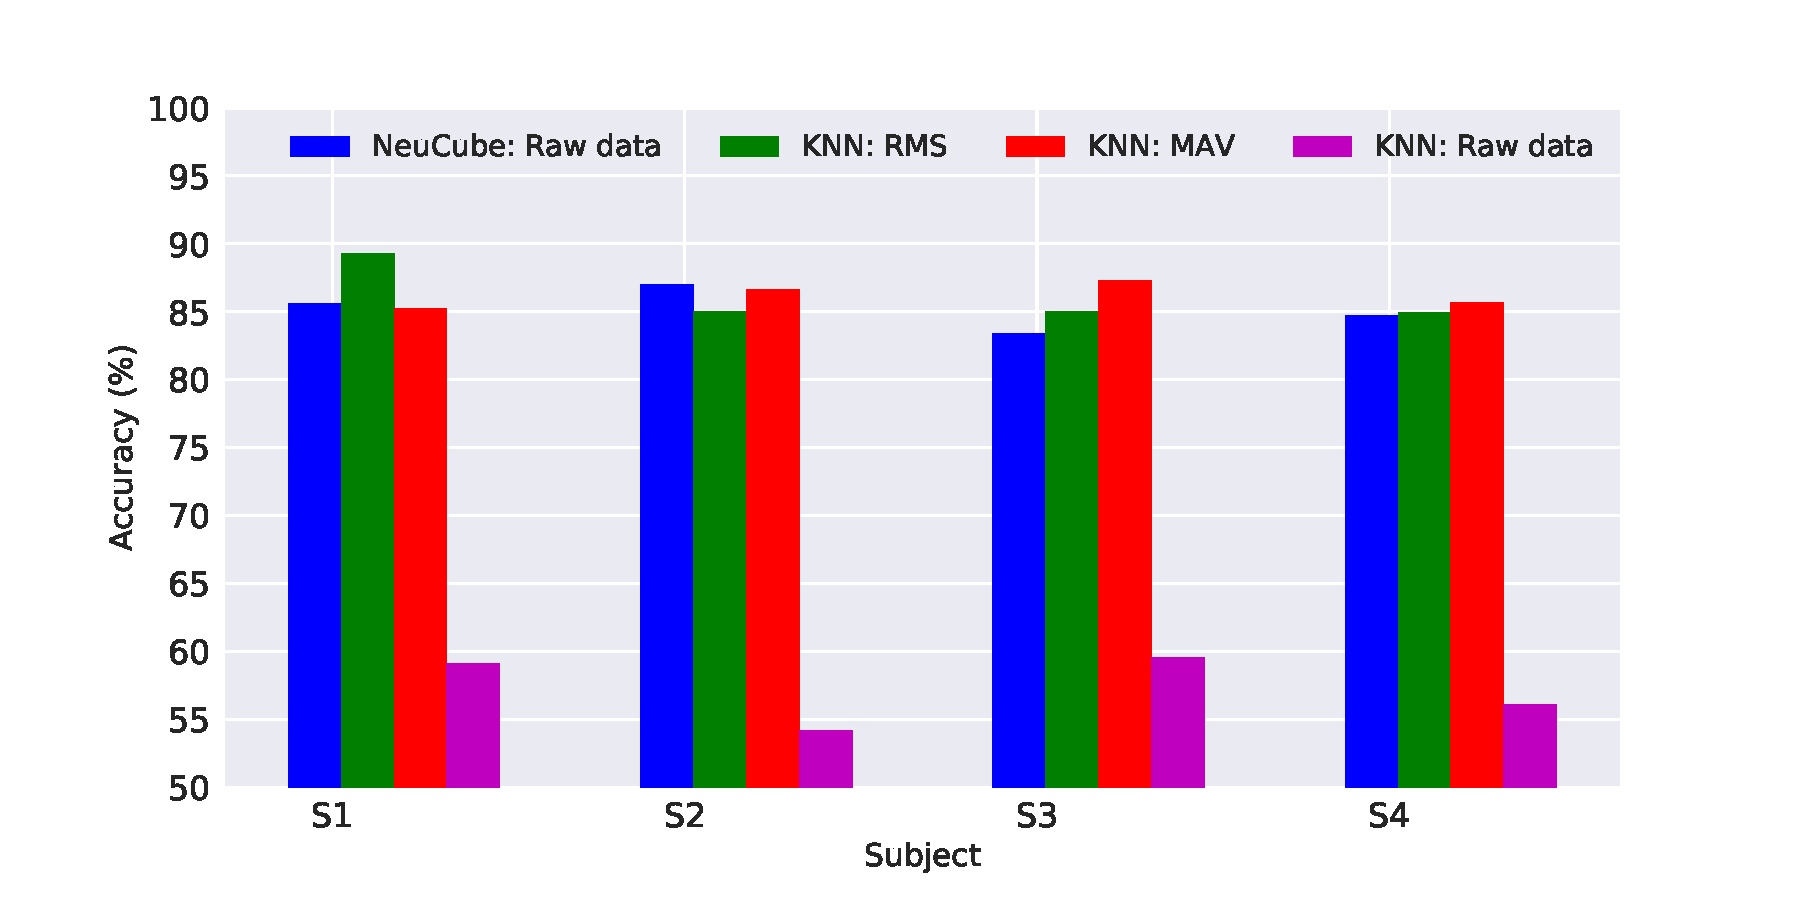
\includegraphics [width=0.85\linewidth]{x.pdf}
    \caption{Comparison of the obtained classification results using NeuCube on the raw data and the KNN with two different feature extraction methods.  
}
    \label{FIG:x.pdf}
\end{figure}
Figure \ref{FIG:x.pdf} shows the variability in achieved results between the different subjects. Overall, S2 scores higher than all the other participants in this classification task with a mean accuracy of 87\%. Mean accuracies of 85.65\% and 84.72\% were obtained from S1 and S4, respectively, whereas S3 performs the worst with a mean accuracy of 83.43\%. As model performance cannot be assessed solely on classification accuracy, precision and recall performance measures were also computed. Results are presented in the confusion matrix in Figure \ref{FIG:confusion_matrix.pdf}. 
\begin{figure}[ht]
    \centering
    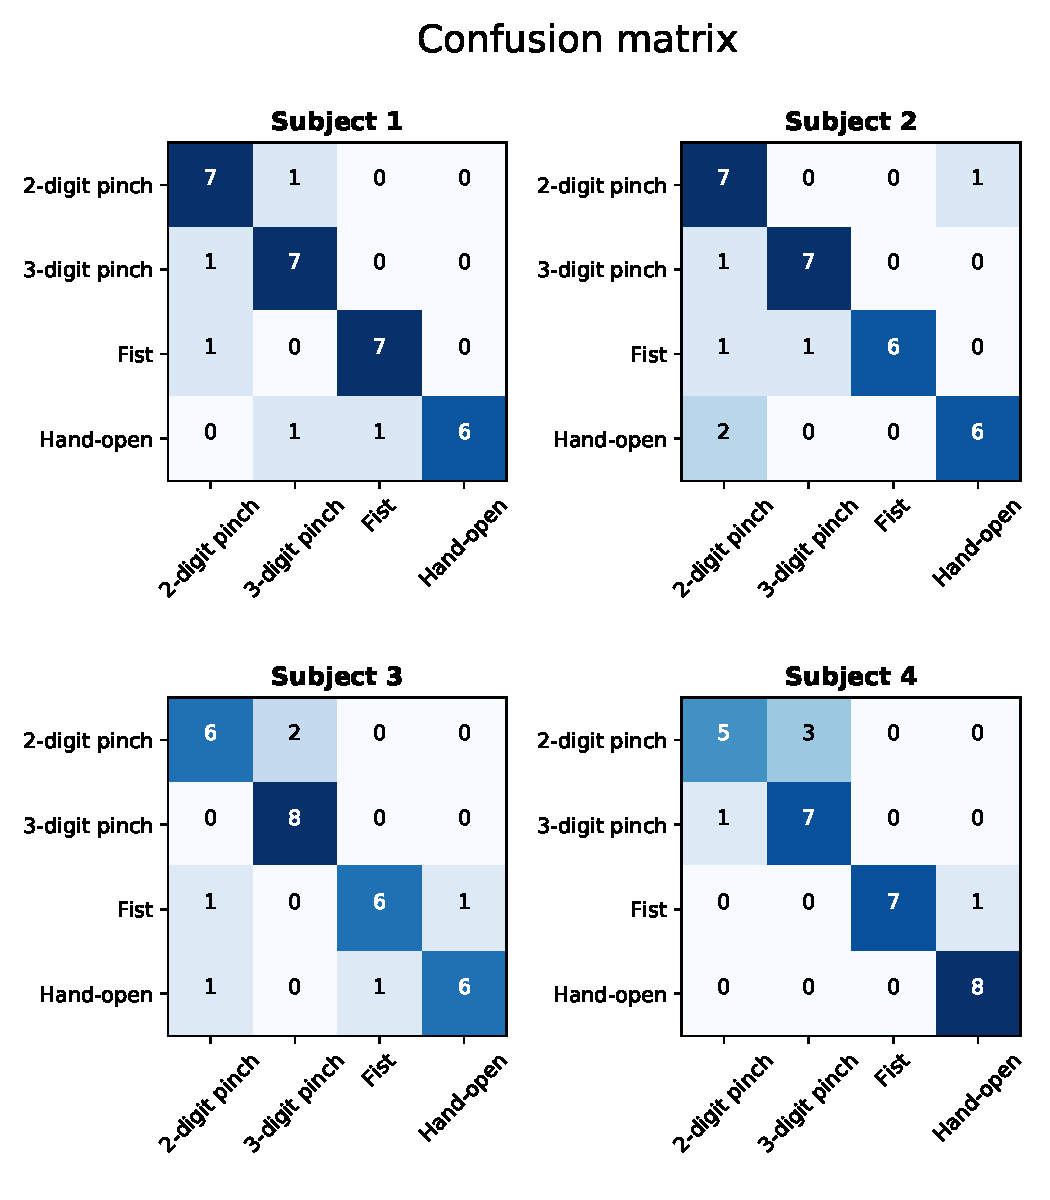
\includegraphics [width=0.6\linewidth]{confusion_matrix.pdf}
    \caption{Confusion matrices for task decoding four hand gestures. Individual confusion matrices are shown for the four subjects. 
}
    \label{FIG:confusion_matrix.pdf}
\end{figure}
The confusion matrix presented in  Figure \ref{FIG:confusion_matrix.pdf} shows that the NeuCube model could classify the fist and the hand-open movements well. However, as shown in Figure \ref{FIG:confusion_matrix.pdf}, the 2-digit pinch and 3-digit pinch movements were confused for some of the subjects.  
\subsubsection{On-line, adaptive, incremental training on new data}
To further test model performance, new inputs were introduced to the trained NeuCube model in real-time. Herein, new online learning was performed and the NeuCube was re-trained and tested in an "online fashion" on new data. Following our experimental paradigm, the first two EMG recording sessions were used for training and validation of the NeuCube model, whereas the third session was used for online prediction. Such a test was designed to evaluate performance of the NeuCube model in real-time scenarios, such as for prosthetic hand control. Overall, a mean accuracy of  $(81\pm 1.4)\%$  was achieved in the test phase across all four subjects. Despite the slight decrease of 4.5\% in the overall (from four subjects) test accuracy compared to the validation case, we can conclude that NeuCube provides stable results, demonstrating the potential of such a model for use in online, adaptive learning and classification tasks. The system can successfully learn and adapt to new data in an on-line, incremental learning mode. The attained accuracies from individual subjects are shown in Figure \ref{FIG:xx.pdf}, reflecting a slight intra-subject variability (variation from 77\% to 83\% in the obtained accuracy). 
\begin{figure}[ht]
    \centering
    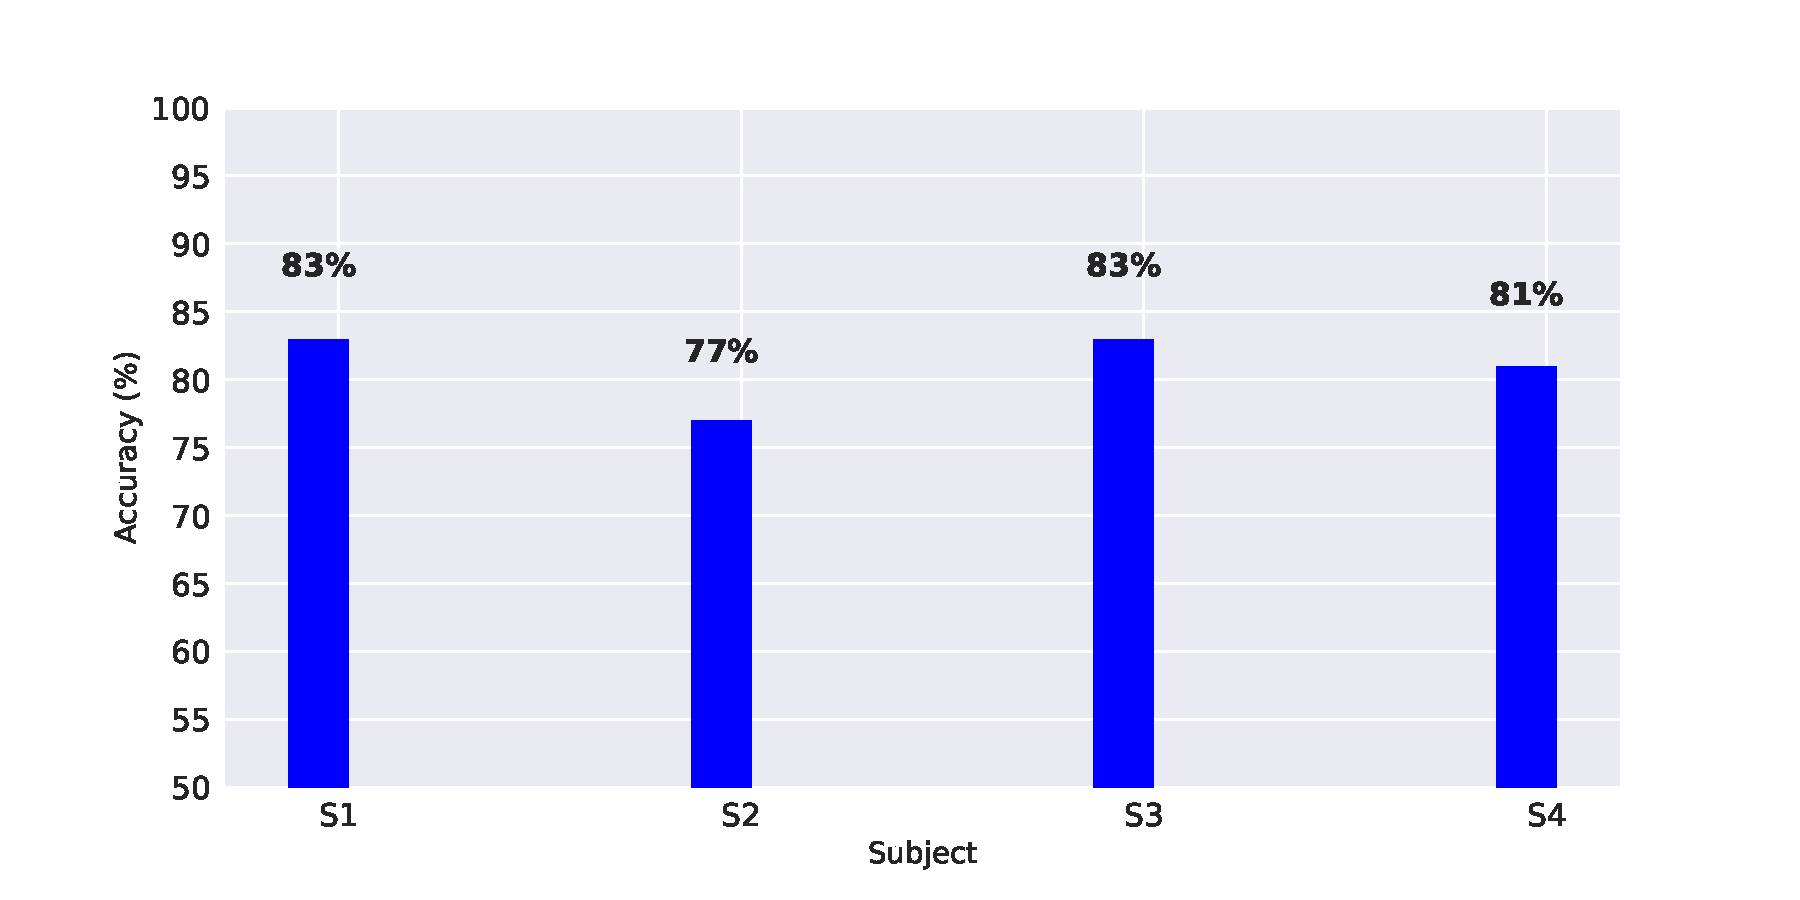
\includegraphics [width=0.85\linewidth]{xx.pdf}
    \caption{Obtained test accuracies for four different subjects. 
}
    \label{FIG:xx.pdf}
\end{figure}
\subsection{Force estimation}
In addition to the recognition of different hand gestures, we also investigated  estimation of the applied force (the force distribution across fingers), when executing the different hand movements. For that, a regressor implemented in the NeuCube software was used. 
Force values from groups of 200 consecutive time points ($\sim 400 ms$) were fed as input into the NeuCube regressor. We wish to mention that the regression was performed similar to the aforementioned classification task. Ben’s Spiker Algorithm (BSA) \cite{37} was used instead of the TD algorithm to encode the force values with a fixed threshold of 0.5. A three-fold cross-validation was performed and the regression results (the true and predicted values of the different trials) are shown in Figure ~\ref{FIG:ForceFigure1.png}. To measure the performance of the validation set, the root mean square error (RMSE)
was used. A RMSE of less than 1.2909 N (rRMSE=18.8\%) was obtained. 
%\usepackage[export]{adjustbox}
\begin{figure}[ht]
    \centering
    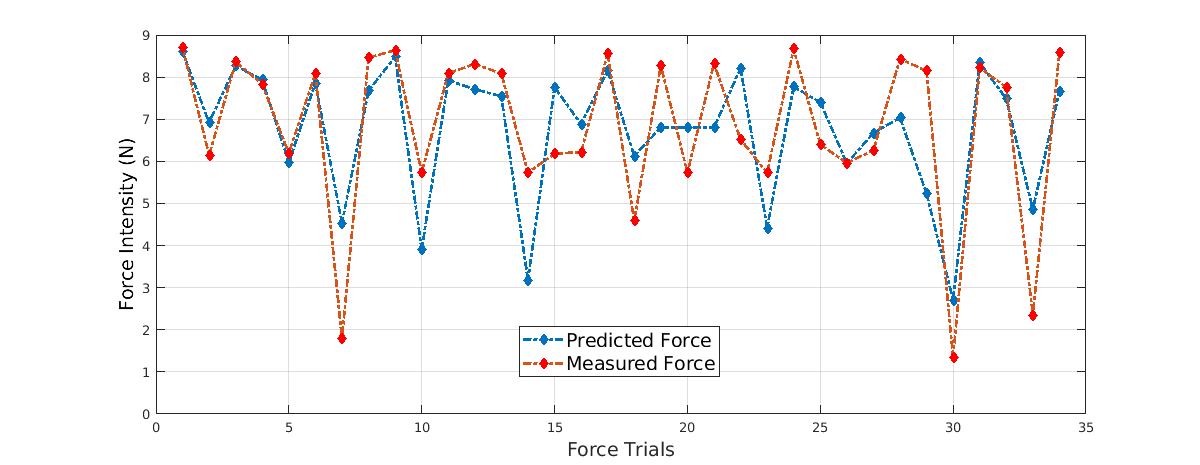
\includegraphics [width=\textwidth]{ForceFigure1.png}
    \caption{Regression results for force estimation.
}
    \label{FIG:ForceFigure1.png}
\end{figure}

%%%%%%%%%%%%%%%%%%%%%%%%%%%%%%%%%%%%%%%%%%%%%%%%%%%%%%%%%
\subsection{Neuromorphic Results}
In this section, we present the overall obtained results of the implementation of the NeuCube model on SpiNNaker for EMG signal decoding. It is important to mention that model calibration remains a major challenge, when testing  a complex system, such as NeuCube. Due to the complex interplay between different stages, and the multitude of parameters involved in the process as well as the probabilistic uncertainty that is introduced with every reservoir creation, it becomes hard to analyze and establish the influence of individual parameters on overall system performance. Hence, the functionality of individual stages of NeuCube was tested first to validate our implementation. Thereafter, the performance of the NeuCube model as an EMG classifier was validated.
\subsubsection{Overall performance of the implemented NeuCube on SpiNNaker}
 The recorded EMG signals collected from four different subjects and sampled at $512\,\text{Hz}$ were used to assess performance. The same preprocessing described before in Section 3.2, was performed on the recorded data. 200 data points were fed into the encoding stage of NeuCube. The input neurons were positioned to maximize the spatial distribution within the reservoir. Noticeably, the different hand poses induced different amplitude patterns on the selected electrodes, which resulted  in a clear and perceivable separation within the reservoir. Although the general class-specific firing pattern was clearly visible during the network's simulation, there
were samples that did not match their respective class pattern, which could be explained by some encoding errors.
Moreover, it is important to highlight that minor parameter changes resulted in a worse classification performance, which shows the importance as well as the effect of network parameters tuning. 
After a very short period of network tuning, a mean accuracy of 75\% across all subjects was achieved in this study. 
%A raster graph, showing the reservoir spike behavior, is presented in Figure \ref{FIG:NeuCubeEMG.png}. 
Overall, obtained results with NeuCube on SpiNNaker are inferior to those obtained on a standard PC (75\% versus 85.5\%). One intuitive reason for that is the higher number of parameters to tune in our NeuCube-SpiNNaker implementation compared to the number of tuning parameters  in the provided Matlab-NeuCube software, tested on a conventional computer. Given that the neuromorphic results were attained without any fine-tuning of the parameters, better performance is undoubtedly achievable with further optimization of the NeuCube's implemented modules.


%\begin{figure}[ht]
    %\centering
    %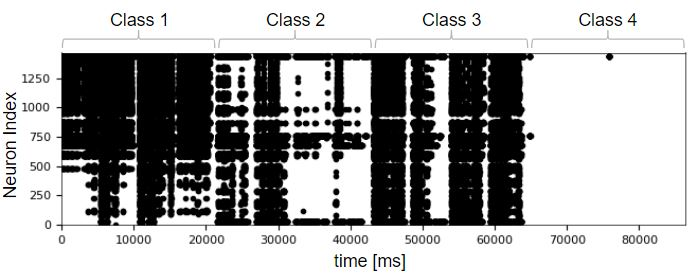
\includegraphics [width=\textwidth]{NeuCubeEMG.png}
    %\caption{Spike raster graph for reservoir activity during presentation of EMG
%samples, clustered by classes for one single subject.
%}
    %\label{FIG:NeuCubeEMG.png}
%\end{figure}

%%%%%%%%%%%%%%%%%%%%%%%%%%%%%%%%%%%%%%%%%%
\section{Discussion}
\subsection{NeuCube is a suitable model for  classification and regression of hand movements and associated forces from raw sEMG data}
In this work, we showed that spiking neural networks, particularly the NeuCube spiking model, could be used to efficiently and accurately decode different hand poses as well as related finger forces from sEMG without hand-crafted features. Several decoding algorithms have been proposed and used in the past \cite{47}. However, the novelty of  this work resides in the direct decoding of recorded signals without extracting discriminative features, thereby allowing for the whole spatio-temporal pattern of hand movement to be learned in a "deep learning mode". Overall, our obtained results do not appear to be in accordance with previous results in \cite{6} where an accuracy of only 68\% was achieved (85.5\% in this work). Aside from the higher number of classes (6 classes) used in that study, another intuitive reason for this difference, is the fine-tuning process of NeuCube's parameters. We observed that these parameters have to be carefully chosen and tuned in order to reach good results, which could explain the difference in the obtained results between the two studies.
Hence, a special attention was given to the selection and the tuning of model parameters during the conduction of this work. Overall, results showed that NeuCube clearly outperformed the classic KNN machine learning algorithm when used without hand-crafted features, and showed comparable performance to the KNN  with well-known discriminitive features for sEMG decoding. Notwithstanding these good results, an intra-variability between the four participants is clearly visible, which is in accordance with previous studies on EMG signal classification \cite{48}. Sweat, slight changes of electrode position during recording, muscle fatigue and the difference between muscle tissues of the participants could drastically decrease the quality of the recorded sEMG signal and lead therefore to a poor performance. 
%As gathering the data is relatively "expensive" and very time-consuming, the number of participants in this study was limited to four. However, a second thorough study with more participants and longer recording sessions, may be required to further investigate the observed intra-variability. 
Furthermore, we also validated the performance of the NeuCube in a real-time scenario, and an overall test accuracy of 80.5\% was achieved. 
%It should be noted, however, that some constraints of the NeuCube software version prevented testing the model with a real prosthetic hand. 
Last, we estimated the applied finger pressure when performing the different hand poses. Despite the good performance (relative error of 18.8\%), it is thought considerable improvements could be achieved. Using more accurate pressure sensors as well as further optimizing the NeuCube regressor's parameters should be addressed in future work. 
\subsection{Successful implementation of the NeuCube model on SpiNNaker neuromorphic hardware}
To complete our investigation of the potential use of spiking models, we implemented the NeuCube on SpiNNaker; a massively parallel neuromorphic system. We validated the overall implementation by successfully classifying the same sEMG data described in the first aforementioned part of this work. Despite such advantages of neuromorphic computing, the use of spiking models on neuromorphic systems to decode time-series signals has been rarely investigated \cite{31, 49}.
First, we encoded the recorded sEMG into spikes. For that, the Ben's Spiker Algorithm (BSA) \cite{37} and the TD algorithm were implemented and compared. Both methods could reliably encode and decode the provided EMG signal. 
%However, we observed that better encoding performance with the TD algorithm could be achieved. As the TD algorithm only considers two consecutive data points and a constant threshold in its spiking decision, the slope that can be encoded and reconstructed by the algorithm is limited to  \textit{inc}\textsubscript{max} = $\frac{\mathrm{threshold}}{\mathrm{time\,step}}$. Therefore, if the threshold is set large, low-frequency high-amplitude components can be encoded but fast and small changes are filtered out. 
In addition, the second stage was designed such that every neuron can conceptually represent some spatio-temporal information from the input data based on its connectivity and spatial arrangement. Overall, the simulation showed that the second stage was successfully validated and a separation between the different EMG classes is clearly visible. Nevertheless, the model was able to classify the presented EMG samples with significantly higher-than-chance accuracy and, thus, the overall system was conceptually validated. It should be noted, however, that the STDP learning rule was disabled in the NeuCube-SpiNNaker implementation. We motivate this choice of turning off the STDP rule,  by a noticeable instability of the network during the simulation when using it. Moreover, it was proven in a previous study \cite{50} that the STDP does not always improve separation but rather leads to a lower separation and high instability if its parameters are set incorrectly. In addition, STDP requires more computation time, more resources and hence a larger SpiNNaker system, which is not suitable for our ultimate prosthetic hand control application.
Aside from that, NeuCube, being brain inspired SNN architecture, has already been used for EEG and fMRI and other brain data modelling \cite{51}. As a result, we can expect that integrating sEMG with EEG data, collected during same data collection process, could improve further the classification and regression results and would allow for more complex movements to be learned. With this regard, one appropriate future test would be to use the hybrid-brain-computer interface (hBCI) by combining EEG and EMG \cite{52}, which may further validate this implementation. Additionally, it is important to highlight that since we have used PyNN \cite{42}, the same implementation should run on other contemporary and future neuromorphic hardware. 
Last, as was shown previously in Section 2.2, the huge number of applications where NeuCube could be used as well as the versatility of such a model could make our proposed approach applicable across different domains. Thus, further investigation of our provided proof-of-concept could spur the use of NeuCube-SpiNNaker implementation in new different applications. 

%\subsection{Limitations and future work}
%In this paragraph, we suggest further steps to improve our NeuCube implementation. First, this initial work should be further used to test the influence of the different parameters in the NeuCube model. For example, the size and shape of the SNN reservoir; the spatial distribution and number of input spike trains/electrodes and the STDP learning parameters should be tested in order to improve the reservoir's performance. 
%%%%%%%%%%%%%%%%%%%%%%%%%%%%%%%%%%%%%%%%%%
\section{Conclusion}
This work is a first attempt to classify four hand poses and estimate related finger forces from raw sEMG signals using the NeuCube spiking model. In addition, we provide a proof of concept of a successful implementation of the proposed spiking model on dedicated neuromorphic hardware. Overall, the NeuCube model showed better performance compared to traditional methods and achieved a mean validation accuracy of 85.2\% and a mean test accuracy of 81\%, across all four subjects. In addition, NeuCube's regressor successfully estimated associated forces with a mean RMSE of 1.2909 N ($\sim 18.8\%$). Furthermore, the neuromorphic NeuCube implementation on the SpiNNaker neuromorphic platform was successfully validated and the implemented model reached a mean classification accuracy of 75\%, when classifying the four classes. Despite the promising results, considerable improvement could be achieved in future work. For instance, additional fine-tuning of the model's parameters  could lead to a better performance. More importantly, the implemented NeuCube model could be transferred to the ultra low-power TrueNorth chip \cite{53}. With a power consumption of less than 70 mW and a compact size, TrueNorth could accelerate the development of the next generation of intelligent prosthetic hands. 


%%%%%%%%%%%%%%%%%%%%%%%%%%%%%%%%%%%%%%%%%%
\vspace{6pt} 

%%%%%%%%%%%%%%%%%%%%%%%%%%%%%%%%%%%%%%%%%%
%% optional
\supplementary{The source code of  the NeuCube-SpiNNaker implementation is made publicly available at  {https://github.com/behrenbeck/NeuCube\_SpiNNaker}, 
All the EMG processing scripts are made publicly available at  \link{https://github.com/gumpy-hybridBCI}.
}



%%%%%%%%%%%%%%%%%%%%%%%%%%%%%%%%%%%%%%%%%%
\authorcontributions{ All authors contributed to this research. ZT designed the research and wrote the paper. JB implemented the NeuCube on SpiNNaker and assisted in writing the paper. CB and ZT did the recording and processing of EMG data as well as the implementation of the NeuCube on a standard computer. CR, OR and NK contributed in the implementation of NeuCube on SpiNNaker and assisted in writing the paper. PC, CR, OR, NK,
SF, GC and JC revised the manuscript. JC supervised this research.}

%%%%%%%%%%%%%%%%%%%%%%%%%%%%%%%%%%%%%%%%%%
\funding{This work was supported in part by Ph.D. grant of the German Academic Exchange Service (DAAD), the German Research Foundation (DFG) and the Technical University of Munich within the funding programme Open Access Publishing. Research and development of the SpiNNaker software stack is supported by the EU ICT Flagship Human Brain Project (HBP SGA2 H2020 785907).}

%%%%%%%%%%%%%%%%%%%%%%%%%%%%%%%%%%%%%%%%%%
\acknowledgments{The authors would like to thank Rémi Laumont and Maxime Kirgo for technical assistance. In addition, we thank Akshay Raj Gollahali and Dr. Josafath Ramos for fruitful discussions.}

%%%%%%%%%%%%%%%%%%%%%%%%%%%%%%%%%%%%%%%%%%
\conflictsofinterest{The authors declare that the research was conducted in the absence of any commercial or financial relationships, which could be construed as a potential conflict of interest.} 



%%%%%%%%%%%%%%%%%%%%%%%%%%%%%%%%%%%%%%%%%%
% Citations and References in Supplementary files are permitted provided that they also appear in the reference list here. 

%=====================================
% References, variant A: internal bibliography
%=====================================
\reftitle{References}

\externalbibliography{yes}
\bibliography{paper.bib}


%% for journal Sci
%\reviewreports{\\
%Reviewer 1 comments and authors’ response\\
%Reviewer 2 comments and authors’ response\\
%Reviewer 3 comments and authors’ response
%}

%%%%%%%%%%%%%%%%%%%%%%%%%%%%%%%%%%%%%%%%%%
\end{document}

